\section{Representing Items}

A database was used to represent items, item sets, students, and student
responses.  A full diagrammatic representation of the database is shown in
Figure~\ref{fig:database}.

\begin{sidewaysfigure}[p!]
 \label{fig:database}
 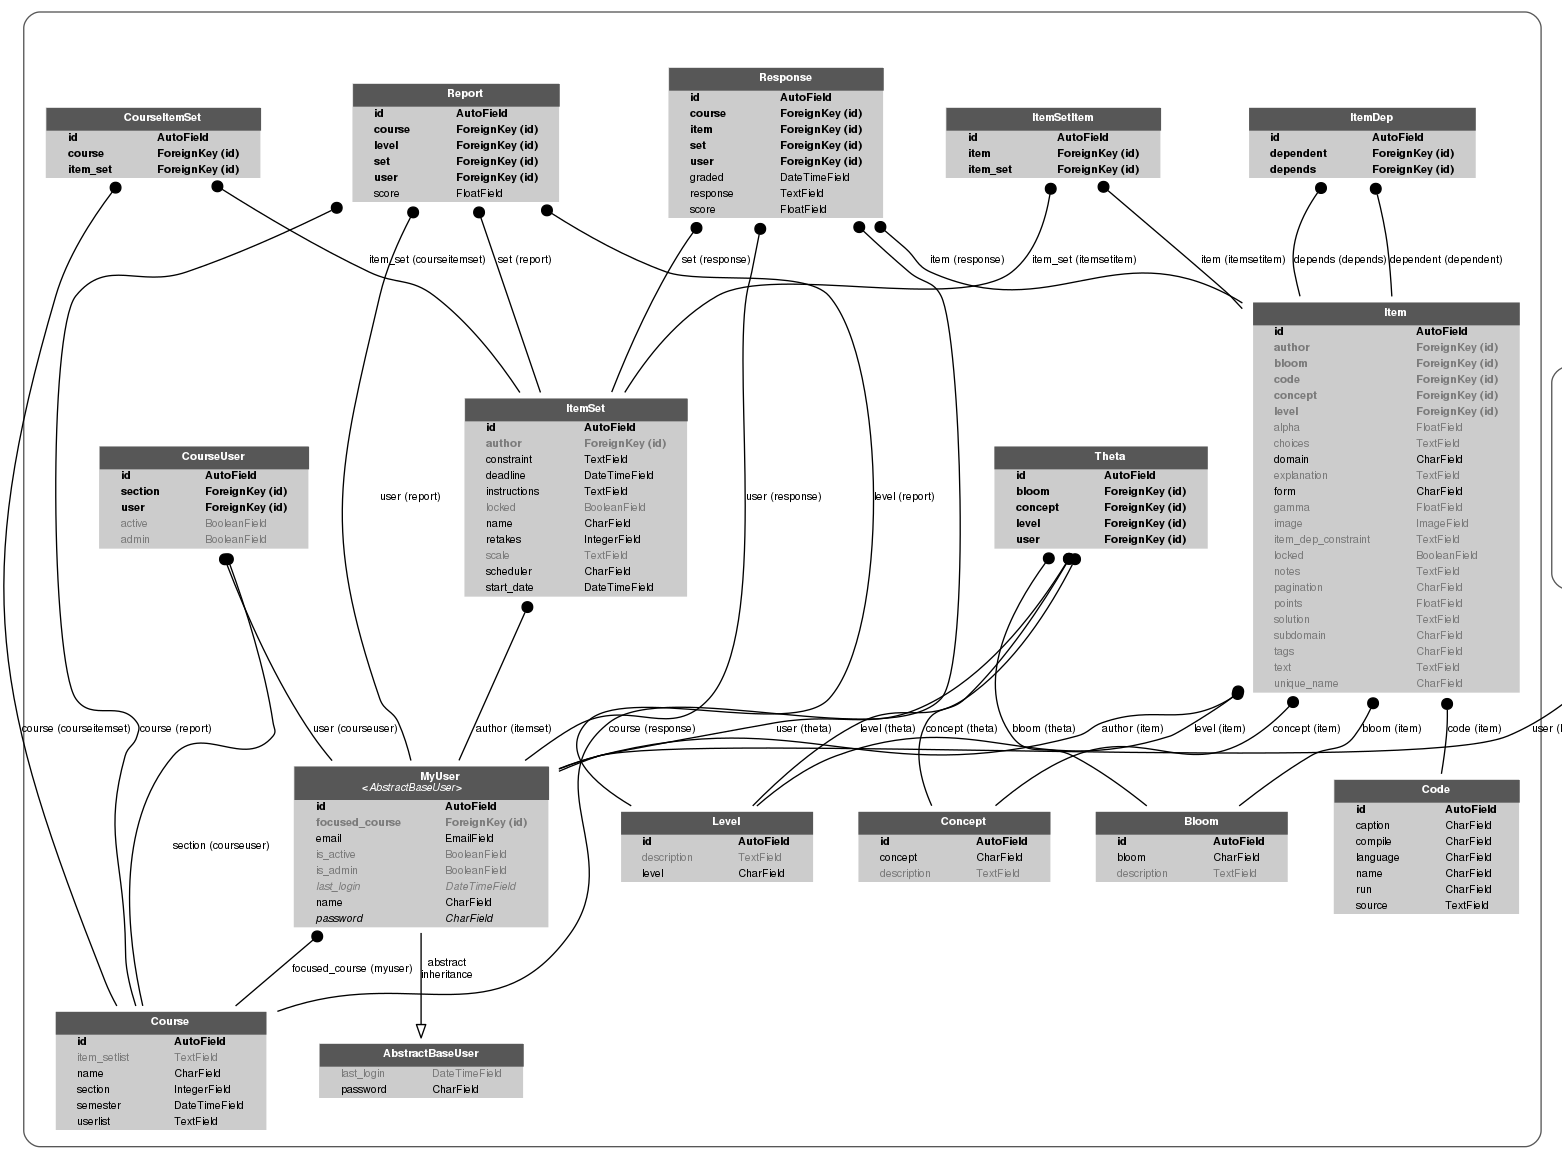
\includegraphics[width=9in]{fig/database.png} 
 \caption{The database layout.}
\end{sidewaysfigure}

The database contains items of the following nature:

\begin{itemize}

  \item \emph{Content}.  These include facts (which may be arranged into
  paragraphs, subsections, and sections), definitions, diagrams, and source
  codes.

  \item \emph{Assessment}.  These include questions, which may be true/false,
  multiple-choice, code writing, code simulation, short answer, and
  freewriting; also Likert scale items.

\end{itemize}

\subsection{Taxonomic Information}

Any output from this database to the student which is intended to solicit input
from the student has the following ordinal dimensions:

\begin{itemize}

  \item \emph{Difficulty}. Following the +/- grading system, difficulties range
  from -3 (very easy) to +3 (very hard), with 0 being medium. As alluded to
  earlier, difficulty determines the probability that a given student in the 
  class will answer the item correctly.

  \item \emph{Bloom level}.  The Bloom levels of cognitive functioning are
  Knowledge, Comprehension, Application, Analysis, Evaluation, and Synthesis.

  \item \emph{Concept}.  Concepts covered in computer science courses; for
  example in a programming course, these may include: Variables, Expressions,
  Control Structures, etc.

\end{itemize}

Any output to the student also has the following categorial dimensions:

\begin{itemize}

  \item \emph{Context}.  A problem may have a domain-specific context, e.g. it
  may be a problem relevant to biology, chemistry, physics, mathematics, etc.

  \item \emph{Type}.  The problem may be true/false, multiple-choice, short
  answer.

\end{itemize}

Each output may also have a dependency list, that is a list of IDs of, or a
rule describing, other output entries which the student should be exposed to
prior to that output.  For this system, Bloom level, subject domain, concept,
and difficulty are dimensions of a test question.  

It is important to note that the dimensions of the data are not necessarily
limited to the above; an exploratory factor analysis (EFA) could be used to
extend the dimensionality of the data semi-automatically.  This functionality
has not been implemented, but there exists a potential for it.

\subsection{Examples of Content Items}

% TODO

\section{Reconciling Bloom's Taxonomy with Item Response Theory}

A popular interpretation of Bloom's cognitive levels is that they are
difficulty levels, and that these difficulty levels are fixed
\cite{newman1988effect,oliver2004course,lord2007moving,
johnson2006bloom,fuller2007developing}.  Knowledge is easy; synthesis is hard.
We will call this the Bloom-equals-difficulty hypothesis.

A creative interpretation of this hypothesis is that per-student difficulty can
be explained in terms of the demotion of Bloom levels.  The synthesis \emph{and
therefore difficult} questions, once the solution is obtained, are reduced to
knowledge \emph{and therefore easy} questions.  Certainly, this is one possible
scenario.  However, it does not explain a student's ability to answer
altogether distinct synthesis problems; this is to suggest students engage the
cognitive functions of synthesis, presumably as an effect of learning the use
of those functions.  To maintain that Bloom equals difficulty would either
require sustaining the view that students are able to pass the questions
because of a demotion of the cognitive functions required (which poses a rather
cynical view of cognition and of education); or else some notion of trait
ability--in particular one which offsets difficulty, allowing an increase in
the probability of passing the question.

The latter option takes the shape of a primeval form of IRT, mapping Bloom
levels to $\beta$.  This is highly convenient for the hypothesis that Bloom
equals difficulty, as it becomes agreeable to evaluation with IRT.  Nontheless,
there are still several issues with the hypothesis.

Consider first that exposure to knowledge and knowledge questions causes an
increase in $\theta$, provided the student acquires the knowledge.  According
to Bloom's theory, this would increase the probability of answering
comprehension questions correctly.  This agrees with the theory.  However,
according to IRT, it would also increase the probability of answering
application questions correctly even if no comprehension-level questions are
asked.  In fact, it is theoretically possible to design tests with sufficient
numbers of knowledge questions to place, for any $\beta$, $\theta-\beta$ much
greater than zero--that is for example to say, asking a sufficient number of
knowledge questions should give the reasonable assurance that application-level
ability is high enough not to bother testing it.

As many educators will no doubt agree, this is not the case. Even if a student
scores exceptionally well on knowledge questions, it gives no such assurance
that the student will score similarly on application-level questions.  Even if
knowledge and application scores are found to be correlated, there may be an
additional underlying factor contributing to both scores (such as
intelligence).  The application level is \emph{qualitatively} different; hence
it needs to be tested in spite of the value of $\theta$.

Second, if the hypotheses is strictly true, then there can exist no
counterexample to the claim.  That is to say that there exists no problem on a
lower Bloom level which is more difficult than a problem on a higher Bloom
level.  To take an example, it would be mistaken to call an application problem
easier than any comprehension problem. 

Counterexmaples with intuitive appeal can be constructed.  Take for-loops for
example.  To ask a student to print out the result of a simple loop which
prints numbers 1 to 10 should present an easy enough task.  This is an
application of the many rules of for-loops, but which does not require creative
synthesis or critical thinking on the part of the student (hence it is an
application problem). 

Consider then asking the student to impose a flowchart over the same code,
including the initialization, condition and update statements and the body of
the loop, and to indicate the start and stop of the loop.  Suppose the student
has seen flowcharts over similar loops before.  This is a test of
comprehension--in particular, comprehension of the internal workings (the
control flow) of the loop.    

The application problem above requires only an intuitive comprehension of the
loop: ``\emph{It prints the sequence from 1 up to 10 in steps of 1}'', the
student may realize.  It demands only shallow comprehension and the rule to be
applied is simple.  In the comprehension problem, on the other hand, a higher
degree of precision in comprehension of the loop is demanded to solve the
problem.  The comprehension problem also depends on mastery of the knowledge,
comprehension, and application of flowchart symbols.  Regardless, explaining
the control flow of the loop in full detail is a more difficult undertaking
than simply printing its output. 

Likewise, it is possible to ask the student to synthesize a loop printing the
first ten powers of two, then ask a comparatively difficult analysis question
in the form of an obfuscated loop code.  Impasses in this situation may be
attributed to a lack of knowledge or comprehension of the constructs used in
the presented code.  In the synthesis problem, the student has the advantage
of using known syntax. 

Third, by Bloom's own admission, it is possible to skip levels for certain
concepts \cite{bloom1956}.  In this case, the ordinality of Bloom levels
breaks down.  A plausible example is given above.  It is possible to teach how
to obtain the numeric sequences printed by for-loops before covering in full
detail the control flow of the loop.  In that particular case, application of
the rule does not depend on comprehension of the code construct.

Alternative interpretations of Bloom levels distinguish between facility or
difficulty and complexity of a problem \cite{hill1981testing,
thompson2008bloom}.  In such interpreations, the cognitive complexity has an
orthogonal relationship to the item difficulty.  The problem with such
interpretations, however, is that they do not readily explain the moderate
correlation that does exist between mean performance and Bloom level
\cite{hill1981testing}.

\subsection{Difficulty vs. Bloom Level}


